\chapter{Cooling Simulations}\label{chap:results}

Before trapping both \ce{Yb^+} and \ce{CHDBrI^+}, we wanted to make sure we are able to cool efficiently only \ce{Yb^+}. We believe that cooling fast the \ce{Yb^+} ions, must help cool fast the \ce{CHDBrI^+} ions. This led us to investigate first how to cool \ce{Yb^+} alone fast, and the main results of this research are in section~\ref{sec:results/laserAngles}. % TODO: If LASER detuning results will be added to this chapter, they should be mentioned in this sentence.

The next thing we checked was... % TODO: Finish the next sentences...

\section{LASER Cooling Intrusion Angle(s) \& Trap Geometry}\label{sec:results/laserAngles}

To date, in our lab, the amount of LASER power we have available for LASER cooling our \ce{Yb^+} is scarce. If obliged to use a single LASER angle, the intuitive choice might be to use the $z$ axis, which is the symmetry axis of the trap, and in which there is also no micromotion. Apparently, the main conclusion from this endeavor is that you \emph{want} to break the symmetry of the trap, and using the $z$ axis is actually the worst choice of them all. The next paragraphs describe how we modeled this, and why we think breaking the symmetry helps.

Our vacuum chamber has only a finite set of windows we can use, so we gave each of them a name, as depicted in figure~\ref{fig:vacuum-chamber-laserAngles}. Each intrusion window is mapped to a $(\theta, \phi)$ pair, as listed in table~\ref{tbl:laserAngles-list}, according to the standard spherical solid angle parametrization depicted in figure~\ref{fig:laserAngles-solid-angle}.

\begin{table}[h]
\centering
\begin{tabular}{lllllll}
\hline
          & $z$       & $r^-$        & $r^+$         & $e^+$      & $e^-$       & $e^*$       \\
\hline
 $\theta$ & $0^\circ$ & $67.5^\circ$ & $112.5^\circ$ & $45^\circ$ & $45^\circ$  & $-45^\circ$ \\
 $\phi$   & $0^\circ$ & $0^\circ$    & $0^\circ$     & $45^\circ$ & $-45^\circ$ & $45^\circ$  \\
\hline
\end{tabular}

\caption{Our available intrusion angles mapping from names to $(\theta, \phi)$ pairs.}
\label{tbl:laserAngles-list}
\end{table}

\begin{figure}
\centering
\begin{subfigure}{0.46\textwidth}
    \centering
    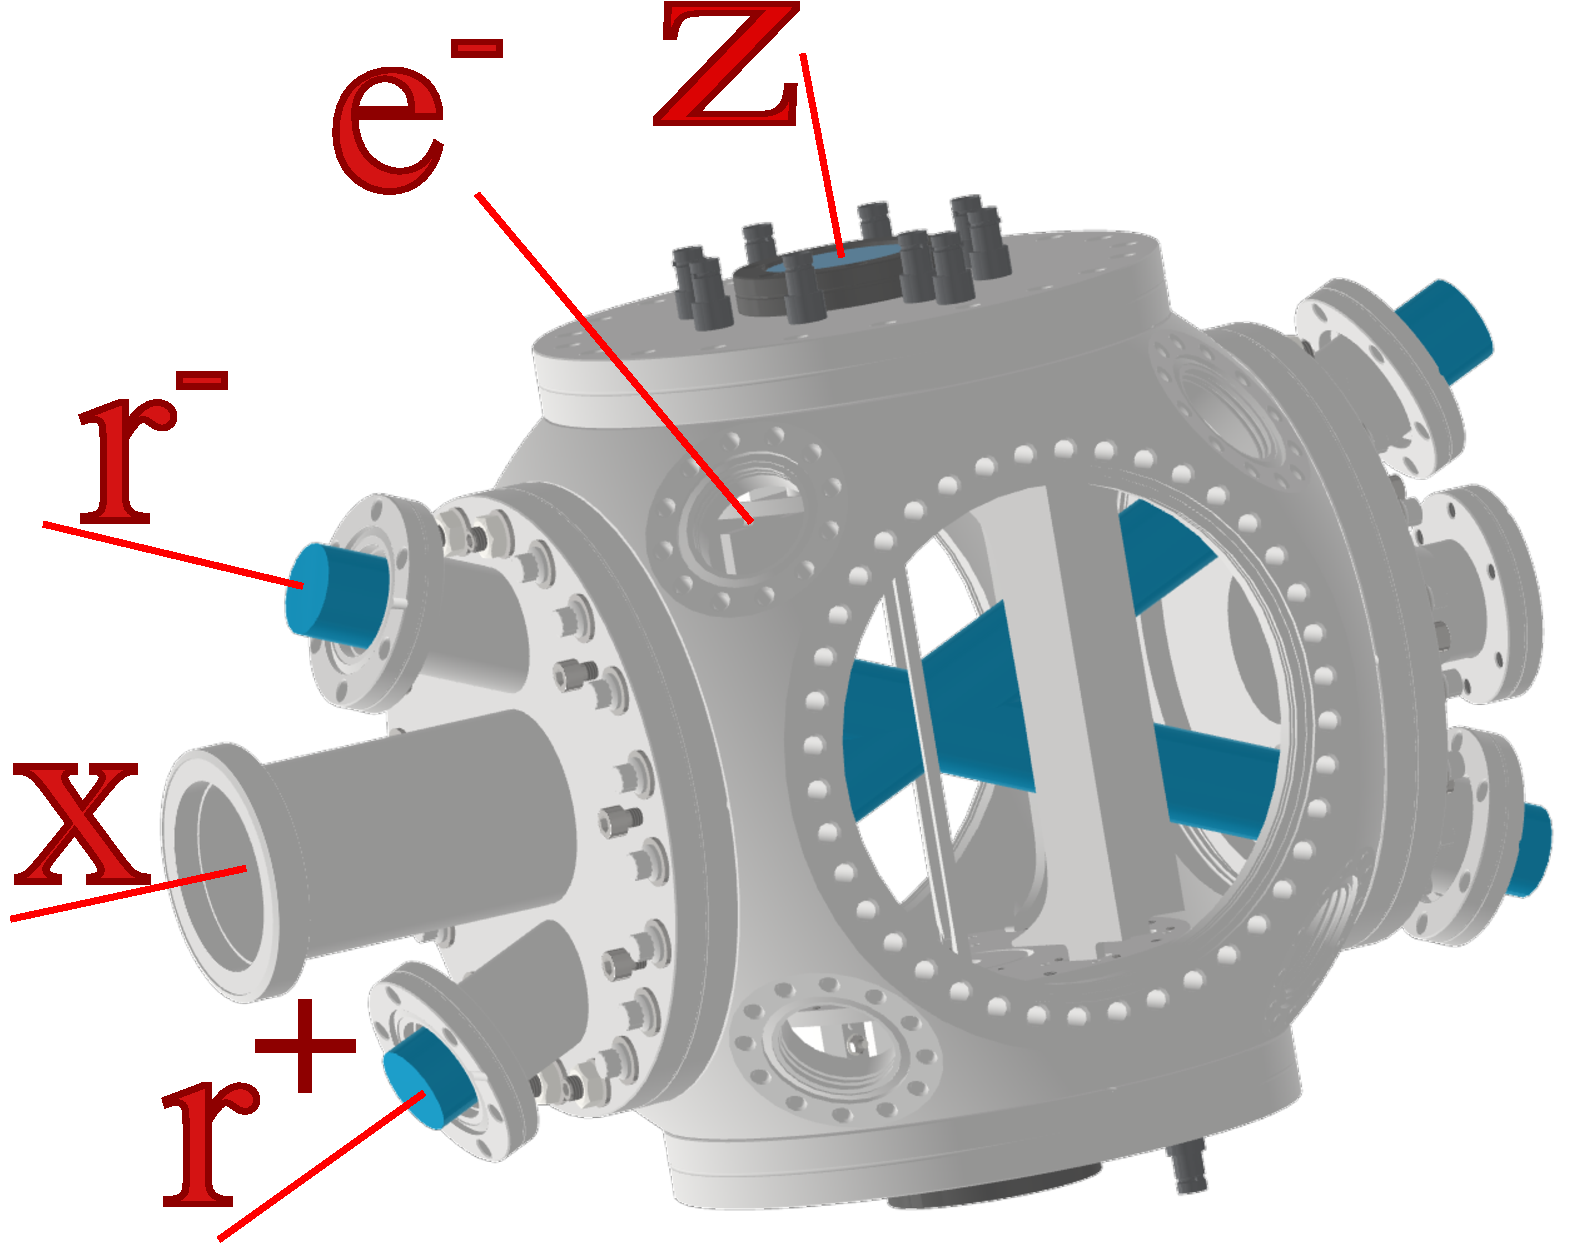
\includegraphics[width=\linewidth]{graphics/vacuum-chamber-windows.pdf}
    \caption{Our vacuum chamber CAD design\cite{ElianaThesis}, annotated with the names we gave of the available windows through which our LASER can intrude.}
    \label{fig:vacuum-chamber-laserAngles}
\end{subfigure}
~
\begin{subfigure}{0.5\textwidth}
    \centering
    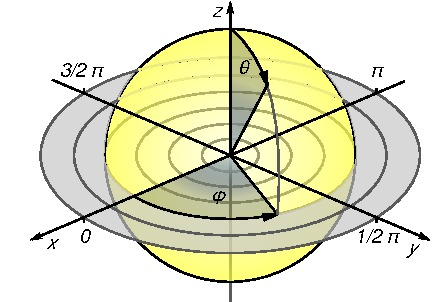
\includegraphics[width=\linewidth]{graphics/ThetaPhiAngles.pdf}
    \caption{Our (standard) solid angles parametrization}
    \label{fig:laserAngles-solid-angle}
\end{subfigure}
\caption{Our LASER intrusion angles parametrization.}
\end{figure}

We simulated cooling of $1000$ \ce{Yb^+} ions, in a trap with frequencies $(f_x, f_y, f_z, f_\mathrm{rf}) = (8.5, 8.5, 1.5, 100)\ \mathrm{kHz}$, with a selection of LASER angles groups. By \emph{group}, I mean either one or more LASERs. In figure~\ref{fig:laserAngles-temperatures}, we can see the significance of the choice of the LASER angles group.

\begin{figure}
    \centering
    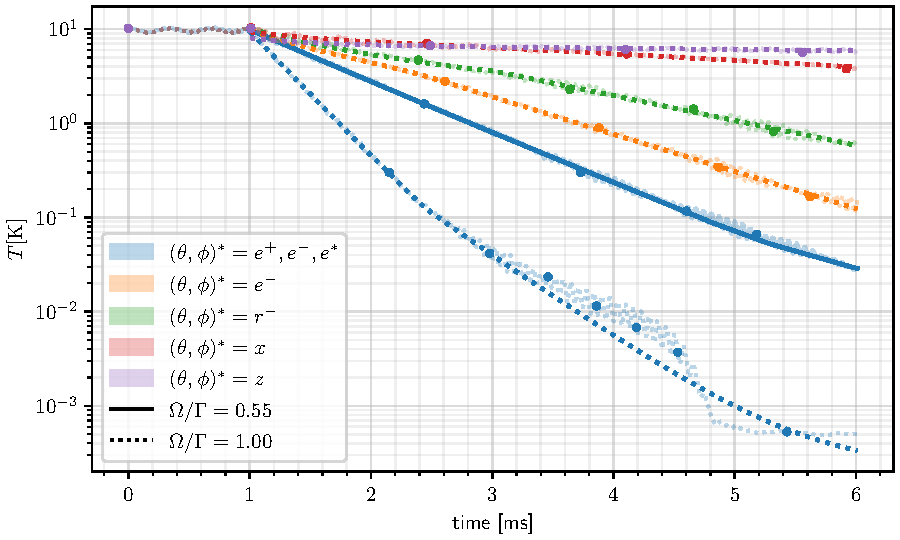
\includegraphics[width=\linewidth]{graphics/laserAngles-dependence--thesis.pdf}
    \caption{Temperatures as a function of time, for several different LASER angles groups. Every LASER entering these simulations had $\Omega/\Gamma = 1$ and $\delta/\Gamma = -2.6$.}
    \label{fig:laserAngles-temperatures}
\end{figure}

Of course using multiple LASERs ($e^+, e^-, e^*$ in this example), all with the same intensities is the most efficient way to cool the ion cloud. However even with a single LASER, you can cool the ion cloud pretty good. Choosing $e^-$ gives slightly better results in comparison to $r^-$, but the later is parallel to the optical table, and hence is slightly easier to setup technically in the lab.

% TODO: Depending on the next sections, a forwarding paragraph should be written. Probably it should state that I chose $r^-$ for many of the scans following.

\section{LASER cooling parameters}

\subsection{Intensity (\(\Omega/\Gamma\)) \& Vacuum Chamber Windows Attenuation}

\subsection{Detuning (\(\delta/\Gamma\))}

\section{\ce{CHDBrI^+} Concentration \& Total \#Ions Dependence}
